\section{Pianificazione} 
	\subsection{Introduzione}
	A fronte dell'analisi dei rischi e della scadenza delle revisioni di avanzamento vi saranno tre periodi durante lo svolgimento del progetto: uno di \textbf{analisi}, uno di \textbf{progettazione e codifica} ed uno di \textbf{incremento e validazione}.
	Per rendere più controllabile lo sviluppo del progetto si è deciso di dividere il lavoro in sei fasi dettagliate, le quali vengono riportate nella seguente tabella con le relative date di inizio e di fine.
		
		\begin{tabella}{!{\VRule}c!{\VRule}c!{\VRule}c!{\VRule}c!{\VRule}}
				
			\intestazionefourcol{Fase}{Abbreviazione}{Data di inizio}{Data di fine}
			
			Analisi & A & 2016/03/01 & 2016/04/18  \\
			Analisi di dettaglio & AD & 2016/04/19 & 2016/04/19  \\
			Progettazione Architetturale & PA & 2016/04/19 & 2016/04/19 \\
			Progettazione di dettaglio e codifica & PDC & 2016/04/19 & 2016/04/19 \\
			Requisiti desiderabili e opzionali & RD & 2016/04/19 & 2016/04/19 \\
			Validazione e verifica & V & 2016/04/19 & 2016/04/19 \\ 
			
			\hiderowcolors
			\caption{Fasi di sviluppo e relative abbreviazioni e date di inizio e fine.}
			
		\end{tabella}
		
	Ogni fase è stata suddivisa in diverse attività che verranno riportate e descritte in un elenco puntato. Successivamente nei diagrammi di \gl{Gantt} si potrà notare come le attività siano state divise lungo l'arco temporale che le varie fasi. Saranno inoltre presenti le \gl{milestones} che coincidono con i giorni in cui dovranno essere consegnati i documenti e i giorni in cui ci saranno le revisioni di avanzamento. 
	\subsection{Fase A}
	Questa fase inizia con la formazione del gruppo e termina il giorno della Revisione dei Requisiti. \\
	Le attività principali di questa fase sono: 
		\begin{itemize}
			\item \textbf{Norme di Progetto}: viene steso il documento \NPdoc in cui saranno elencate e descritte le norme da seguire durante tutto lo svolgimento del progetto indipendentemente dal capitolato scelto;
			\item \textbf{Piano di Progetto}: viene steso il documento \PPdoc per pianificare dettagliatamente i tempi e i costi del progetto;
			\item \textbf{Studio di Fattibilità}: viene steso il documento \SFdoc che riporta l'analisi che ha portato il gruppo a scegliere il capitolato C2.
			\item \textbf{Analisi dei Requisiti}: viene steso il documento \ARdoc in cui viene svolta un'analisi molto più approfondita di quella svolta in \SFdoc. Vengono elencati e descritti i casi d'uso e i requisiti del prodotto che si andrà a sviluppare;
			\item \textbf{Piano di Qualifica}: viene steso il documento \PQdoc che riporta che obiettivi di qualità si è prefissato il gruppo;
			\item \textbf{Glossario}: viene steso il \Gldoc il quale riporta la descrizione dei termini presenti nei vari documenti che potrebbero causare ambiguità nel lettore.
			
		\end{itemize}
		\subsubsection{Diagramma di Gantt delle attività}
		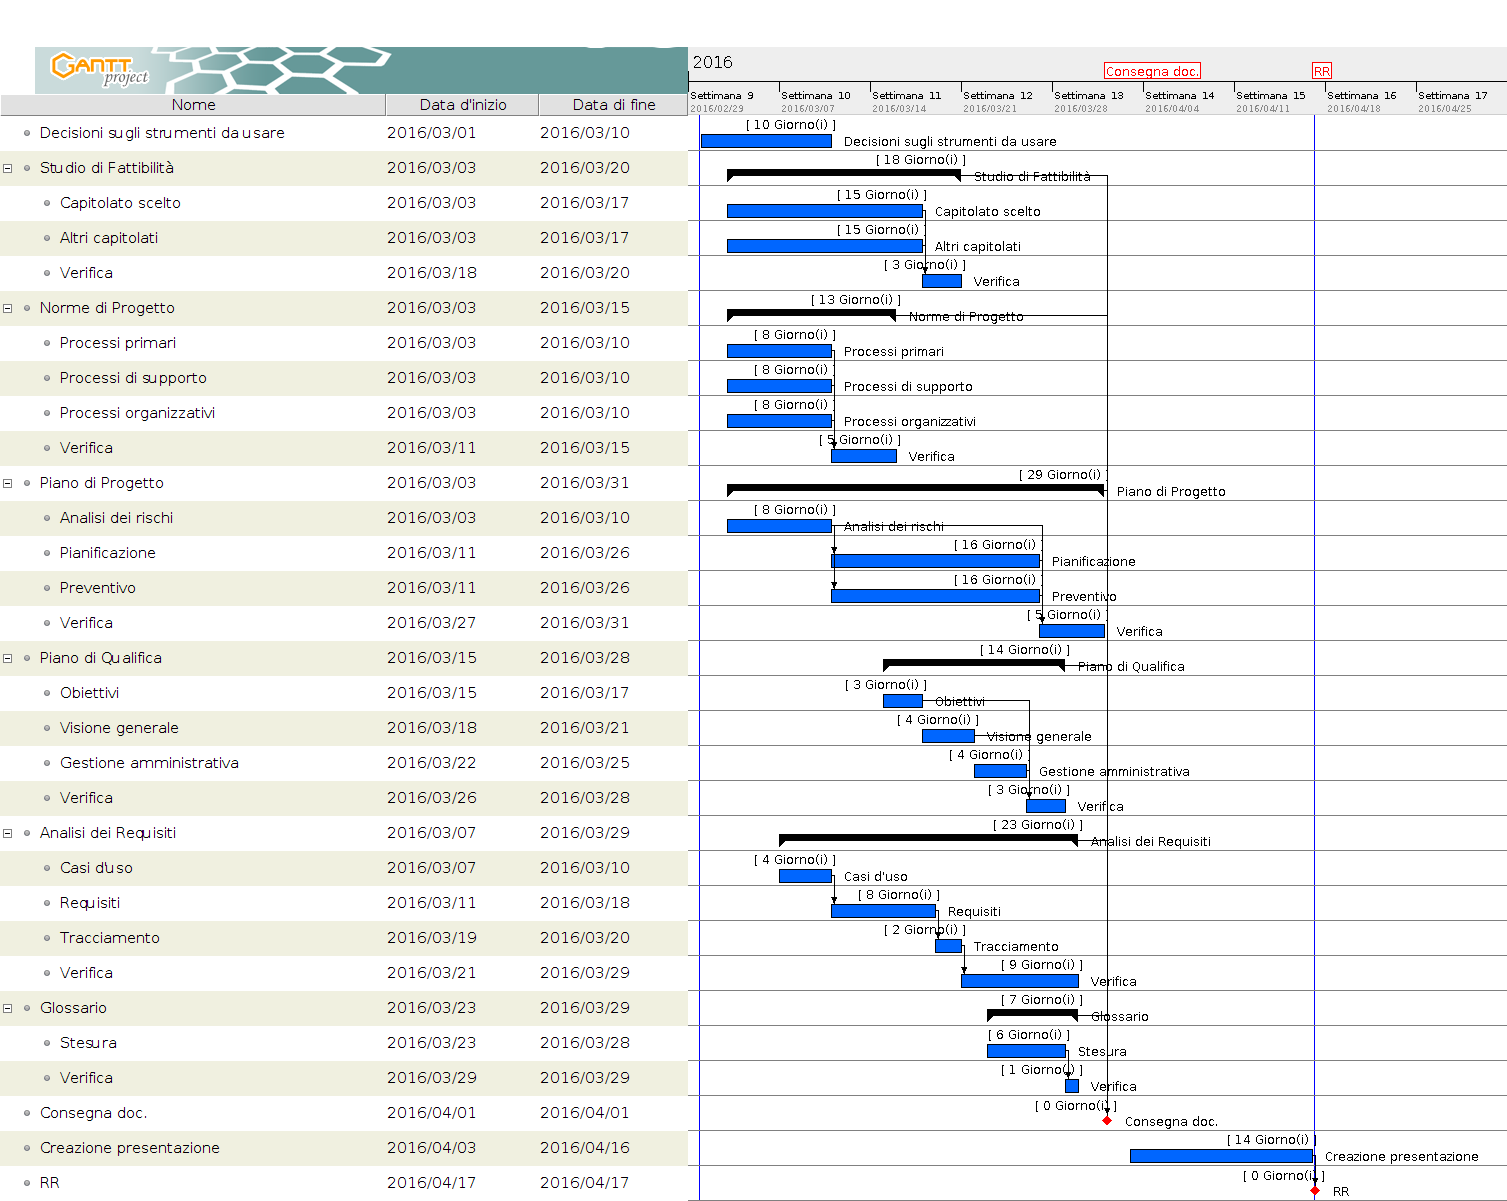
\includegraphics[scale=0.3]{img/A.png} 
		
		
	\subsection{Fase AD}
		\begin{itemize}
			\item \textbf{Individuazione strumenti} 
			\item \textbf{Norme di Progetto}
			\item \textbf{Piano di Progetto}
			\item \textbf{Studio di Fattibilità}
			\item \textbf{Analisi dei Requisiti}
			\item \textbf{Piano di Qualifica}
			\item \textbf{Glossario}
		\end{itemize}
		\subsubsection{Diagramma di Gantt delle attività}
		
	\subsection{Fase PA}
		\begin{itemize}
			\item \textbf{Individuazione strumenti} 
			\item \textbf{Norme di Progetto}
			\item \textbf{Piano di Progetto}
			\item \textbf{Studio di Fattibilità}
			\item \textbf{Analisi dei Requisiti}
			\item \textbf{Piano di Qualifica}
			\item \textbf{Glossario}
		\end{itemize}
		\subsubsection{Diagramma di Gantt delle attività}
		
	\subsection{Fase PDC}
		\begin{itemize}
			\item \textbf{Individuazione strumenti} 
			\item \textbf{Norme di Progetto}
			\item \textbf{Piano di Progetto}
			\item \textbf{Studio di Fattibilità}
			\item \textbf{Analisi dei Requisiti}
			\item \textbf{Piano di Qualifica}
			\item \textbf{Glossario}
		\end{itemize}
		\subsubsection{Diagramma di Gantt delle attività}
		
	\subsection{Fase RD}
		\begin{itemize}
			\item \textbf{Individuazione strumenti} 
			\item \textbf{Norme di Progetto}
			\item \textbf{Piano di Progetto}
			\item \textbf{Studio di Fattibilità}
			\item \textbf{Analisi dei Requisiti}
			\item \textbf{Piano di Qualifica}
			\item \textbf{Glossario}
		\end{itemize}
		\subsubsection{Diagramma di Gantt delle attività}
		
	\subsection{Fase V}
		\begin{itemize}
			\item \textbf{Individuazione strumenti} 
			\item \textbf{Norme di Progetto}
			\item \textbf{Piano di Progetto}
			\item \textbf{Studio di Fattibilità}
			\item \textbf{Analisi dei Requisiti}
			\item \textbf{Piano di Qualifica}
			\item \textbf{Glossario}
		\end{itemize}
		\subsubsection{Diagramma di Gantt delle attività}
	
